% This is a simple, plain Latex template package for the creation of Bachelor's and 
% Master's theses.
% The template is tailored to the specific needs of engineering students pursuing a degree
% at the University of Lübeck.
%
% For copyright information, see the accompanying LICENSE file.
%
% The current version of this template can always be found at
%
%    https://github.com/gonike/thesis-template
%
% Eike Petersen, May 2016.
%

\documentclass[11pt, a4paper, headsepline, BCOR = 1cm]{scrbook}
% BCOR = Binding correction. Adjusts inner page margin for bound books.
% headsepline produces a horizontal line under chapter title on page headers

%%%%% General packages & Utilities

% Allow for German "Umlaute"
% Note that for this to work, all files containing Umlaute must be saved in the UTF-8 file format!
\usepackage[T1]{fontenc}
\usepackage[utf8]{inputenc}

% Tables
\usepackage{booktabs}

% Make todo notes in the thesis.
% Simply change the status to "final" to suppress printing of the notes and their list.
\usepackage[status=draft]{fixme}

% Useful in defining custom shortcut commands
\usepackage{xspace}

% Load english and german language hyphenation and options.
% The language put last here is selected as the main language for the document,
% specifying keywords such as Table of Contents / Inhaltsverzeichnis, etc.
\usepackage[ngerman, english]{babel}
\usepackage{csquotes}


%%%%% Style

% Font type
\usepackage{lmodern}

% Line spacing
\usepackage{setspace}
%\singlespacing
\onehalfspacing
%\doublespacing



%%%%% Graphics packages

\usepackage{graphicx}

%% add subfolder containing figures to the graphics path
\graphicspath{{figures/}}

% Subfigures
\usepackage{caption}
\usepackage{subcaption}

% Powerful package for programmatically producing nice vector graphics
\usepackage{tikz}

% Package for easily drawing electrical circuits (uses tikz)
\usepackage[european]{circuitikz}

% Package for creating plots in latex using tikz internally
\usepackage{pgfplots}
\pgfplotsset{compat=1.11}
\usepgfplotslibrary{units}



%%%%% Referencing, Glossary, Bibliography

% Allow for cross-referencing other parts of this documents
% -- hidelinks prevents ugly red boxes around clickable items. Alternatively, these could be styled differently.
% -- pdfusetitle adds author and title information to meta data
\usepackage[hidelinks, pdfusetitle]{hyperref}

% Easier cross-referencing, using the \cref and \Cref commands
\usepackage{cleveref}

% Glossaries must be loaded after hyperref
\usepackage[style = long, nolist, acronym, nonumberlist, nopostdot, toc]{glossaries}
\newglossary{symbols}{sym}{sbl}{List of Mathematical Symbols}
\makenoidxglossaries

% Bibliography
\usepackage[backend=biber, style=ieee, sorting=nyt]{biblatex}
% Change the separator between title and subtitle of a book from comma to colon
\renewcommand{\subtitlepunct}{\addcolon\addspace}
% Make the space between author names and actual reference in the \textcite
% command non-breakable.
\renewcommand\namelabeldelim{\addnbspace}
\addbibresource{references.bib}

% Add lines to table of contents for list of figures, tables, etc. and for bibliography.
% Alternatively (e.g. when not using a KOMA document class), this could be achieved by 
% adding
%     \addcontentsline{toc}{chapter}{List of Figures}
% before \listoffigures, and similarly for the others.
\KOMAoptions{
  listof=totoc,
  bibliography=totoc
}



%%%%% Maths and computer science packages

\usepackage{amsmath}
\usepackage{amsthm}
\usepackage{amsfonts}
\usepackage{mathtools}

% introduce new type of theorems (uses amsthm package)
\newtheorem{lemma}{Lemma}

% Improvement of \left and \right due to 
% http://tex.stackexchange.com/questions/2607/spacing-around-left-and-right
\usepackage{mleftright}

% Produce pseudo code sections
% See http://tex.stackexchange.com/a/230789/64293 for a discussion of the various
% packages available for this task.
\usepackage{algorithm}
\usepackage{algpseudocode}

% Correctly display SI units
\usepackage{siunitx}



%%%%% Abbreviations and macros

% Order must be first macros then glossary, since the latter uses the former

\newcommand*\submitdate{1. April 2020}


%% ABBREVIATIONS & MACROS

\newcommand{\swname}[1]{\texttt{#1}}


%% GENERAL MATHS STUFF

\newcommand*{\diff}{\mathrm{d}}
\newcommand*{\pdiff}[0]{\partial}
\newcommand*{\dd}[2][]{\frac{\pdiff #1}{\pdiff #2}}


%% CHAPTER MATERIALS AND METHODS

\newcommand*{\vel}{v}
\newcommand*{\loc}{x}
\newcommand*{\acc}{a}
\newcommand*{\mass}{m}
\newcommand*{\force}{f}


%% CHAPTER CONCEPT

\newcommand*{\Bfun}{B}
\newcommand*{\Afun}{A}




%%%%% Emacs-related stuff
%%% Local Variables: 
%%% mode: latex
%%% TeX-master: "main"
%%% End: 

\loadglsentries{glossary}



%%%%% Emacs-related stuff
%%% Local Variables: 
%%% mode: latex
%%% TeX-master: "main"
%%% End: 


\begin{document}

\frontmatter
\KOMAoptions{twoside = false}
\begin{titlepage}

  
\includegraphics[width=8cm]{logo_ime}

  \vspace{0.8cm}

  \begin{center}

    \LARGE
    Blind Source Separation on Surface

    Electromyographic Measurements

    \vspace{1cm}

    \Large

    Blinde Quellentrennung an Messungen des Oberflächen-Elektromyogramms

    \vspace{0.8cm}

    \large

    \textbf{Masterarbeit} 

    im Rahmen des Studiengangs Informatik der Universität zu Lübeck

    \vspace{0.8cm}
    
    Vorgelegt von

    \textbf{Maxima Musterfrau}

    \vspace{0.8cm}

    Ausgegeben und betreut von

    Prof. Dr. Awesome Scientist

    \vspace{0.8cm}

    Mit Unterstützung von

    Lucky PhD Student

    \vspace{0.8cm}

    Diese Arbeit ist im Rahmen von Arbeiten 

    bei der Firma PerfectSolutions GmbH entstanden.
    
    \vspace{1.3cm}

    Lübeck, den \submitdate

  \end{center}

\end{titlepage}
\KOMAoptions{twoside}

%%%%% Emacs-related stuff
%%% Local Variables: 
%%% mode: latex
%%% TeX-master: "../../main"
%%% End: 

\cleardoublepage

\KOMAoption{headsepline}{false}

\subsection*{Eidesstattliche Erklärung}
Hiermit erkläre ich an Eides statt, dass ich die vorliegende Arbeit ohne unzulässige Hilfe Dritter und ohne die Benutzung anderer als der angegebenen Hilfsmittel selbst\-ständig verfasst habe; die aus anderen Quellen direkt oder indirekt übernommenen Daten und Konzepte sind unter Angabe des Literaturzitats gekennzeichnet.

\vspace{2cm}

Lübeck, den \submitdate


%%%%% Emacs-related stuff
%%% Local Variables: 
%%% mode: latex
%%% TeX-master: "../../main"
%%% End: 

\cleardoublepage

\subsection*{Abstract}
Short summary of your thesis goes here.
Must be translated into german.


%%%%% Emacs-related stuff
%%% Local Variables: 
%%% mode: latex
%%% TeX-master: "../../main"
%%% End: 

\cleardoublepage

\subsection*{Kurzzusammenfassung}
An diese Stelle kommt eine Kurzzusammenfassung der Arbeit.
Dies sollte eine Übersetzung des englischen Abstracts sein.

%%% Local Variables: 
%%% mode: latex
%%% TeX-master: "../../main"
%%% End: 

\cleardoublepage

\KOMAoption{headsepline}{true}

\tableofcontents

\mainmatter

\chapter{Introduction}
\label{chap:intro}

Here comes your introduction.

\fxnote{This is a FixMe Note that tells you to complete the introduction of your thesis.}

\section{Previous Works}
This section should contain a quick overview of the previous results of other researchers or students relevant to your thesis project.

\section{Thesis outline}
\Cref{chap:materials-and-methods} presents...
The central concept proposed in this thesis is outline in \cref{chap:concept}.
Consequently, the result of testing the concept experimentally are proposed in \cref{chap:results}....


%%%%% Emacs-related stuff
%%% Local Variables: 
%%% mode: latex
%%% TeX-master: "../../main"
%%% End: 

\chapter{Materials and Methods}
\label{chap:materials-and-methods}

This chapter deals with background information relevant for your thesis, including physiological background, existing research on the topic, and mathematical and other preliminaries required to understand the novel concepts presented in the following chapter.


\section{Getting started with Latex}
\label{sec:getting-started-with}

To get started with Latex, you need...
\begin{itemize}
\item a tool that generates a PDF file out of a bunch of *.tex and *.bib files.
Under Windows, this is typically \swname{MikTex} (\url{http://miktex.org/download}).
\item a text editor. This can be as simple as \swname{Notepad++}(\url{https://notepad-plus-plus.org/}), but many would recommend an IDE that provides further convenience features. \swname{TexMaker}(\url{http://www.heise.de/download/texmaker.html}) and \swname{TexStudio}(\url{http://www.texstudio.org/}) are two well-known examples.
\end{itemize}
If you have these two installed on your PC, you're ready to go!

There is a wealth of references and tutorials on the internet that deal with Latex.
What follows is a small list compiled based on my personal preferences.
\begin{itemize}
\item ShareLatex currently provides - to my taste - the best introduction and reference on a number of Latex-related topics: \url{https://www.sharelatex.com/learn}.
\item Latex-Wikibooks often prove useful if you're really looking for a reference of the available symbols, e.g. \url{https://en.wikibooks.org/wiki/LaTeX/Mathematics} or \url{https://en.wikibooks.org/wiki/LaTeX/Tables}.
\item There is a neat little online tool available, which provides users with hints on available Latex commands based on the user's drawing of the desired symbol: \url{http://detexify.kirelabs.org/classify.html}.
\item Malte Schmitz from the Uni Lübeck also provides good introductory material in German: \url{http://www.mlte.de/layout}.
\end{itemize}

\section{Thesis writing strategies}

\subsection{Have a plan before you start}
Before starting to write any paragraph of full text in your thesis, you should now to a high degree of detail the contents of every chapter of your thesis.
Otherwise, you will find yourself rewriting and maybe even dumping large parts of what you wrote earlier.
Ideally, create a detailed outline of the story you want to tell in your thesis, and make it clear to yourself how each chapter contributes to this central story.
It also helps to collect and create explanatory figures early on that can help you identify the concepts you need to explain in your thesis.

\subsection{Reproducible research}
\emph{Reproducible research} is a term that has gained a lot of attention recently.
It describes research that is easily reproducible by yourself, as well as others.
Note that many common research practices are not easily reproducible at all, e.g.
\begin{itemize}
\item Saving figures you created somehow \swname{Matlab}, without saving a script file that can reproduce this figure.
\item Somehow modifying measured data (e.g. performing a smoothing operation), without saving anywhere the details of what you did.
\item Changing a results table in your report according to new results - but a week later you can't recall how you came to these results.
\end{itemize}
Keeping your work reproducible is not only useful for others, but also (and especially) for yourself: It makes sure that all parts of your work (data, analysis, report, etc.) are always in sync.
Furthermore, you can, e.g., easily update all figures in your thesis a week before the deadline - which may be a nightmare if you created all of these figures manually and cannote reproduce them easily.
A good introduction to the steps required to keep your work reproducible can be found at \url{http://kbroman.org/steps2rr/}.

\section{Preparing a scientific presentation}
The following is just a quick list compiled to help in creating good scientific presentations.
\begin{itemize}
\item \url{http://www.the-scientist.com/?articles.view/articleNo/28818/title/Pimp-your-PowerPoint/}
\item \url{http://www.northwestern.edu/climb/resources/oral-communication-skills/creating-a-presentation.html}
\item \url{http://www.nextscientist.com/improve-presentation-skills-of-phd-students/}
\end{itemize}




%%%%% Emacs-related stuff
%%% Local Variables: 
%%% mode: latex
%%% TeX-master: "../../main"
%%% End: 

\chapter{Concept}
\label{chap:concept}

This chapter describes the novelty that you have created during the making of your thesis.
This novelty might be an experimental apparatus, a novel algorithm, or a thorough analysis of something.
You may here reuse the background information presented in the previous chapter.

\section{Figures in Latex}
\Cref{fig:sfap-schematic} shows a schematic of the geometry of of \gls{sfap} detection.
Note the extensive figure caption: many readers will first skim through your thesis and look at the figures, which should hence be as self-explanatory as possible.
\begin{figure}
  \centering
  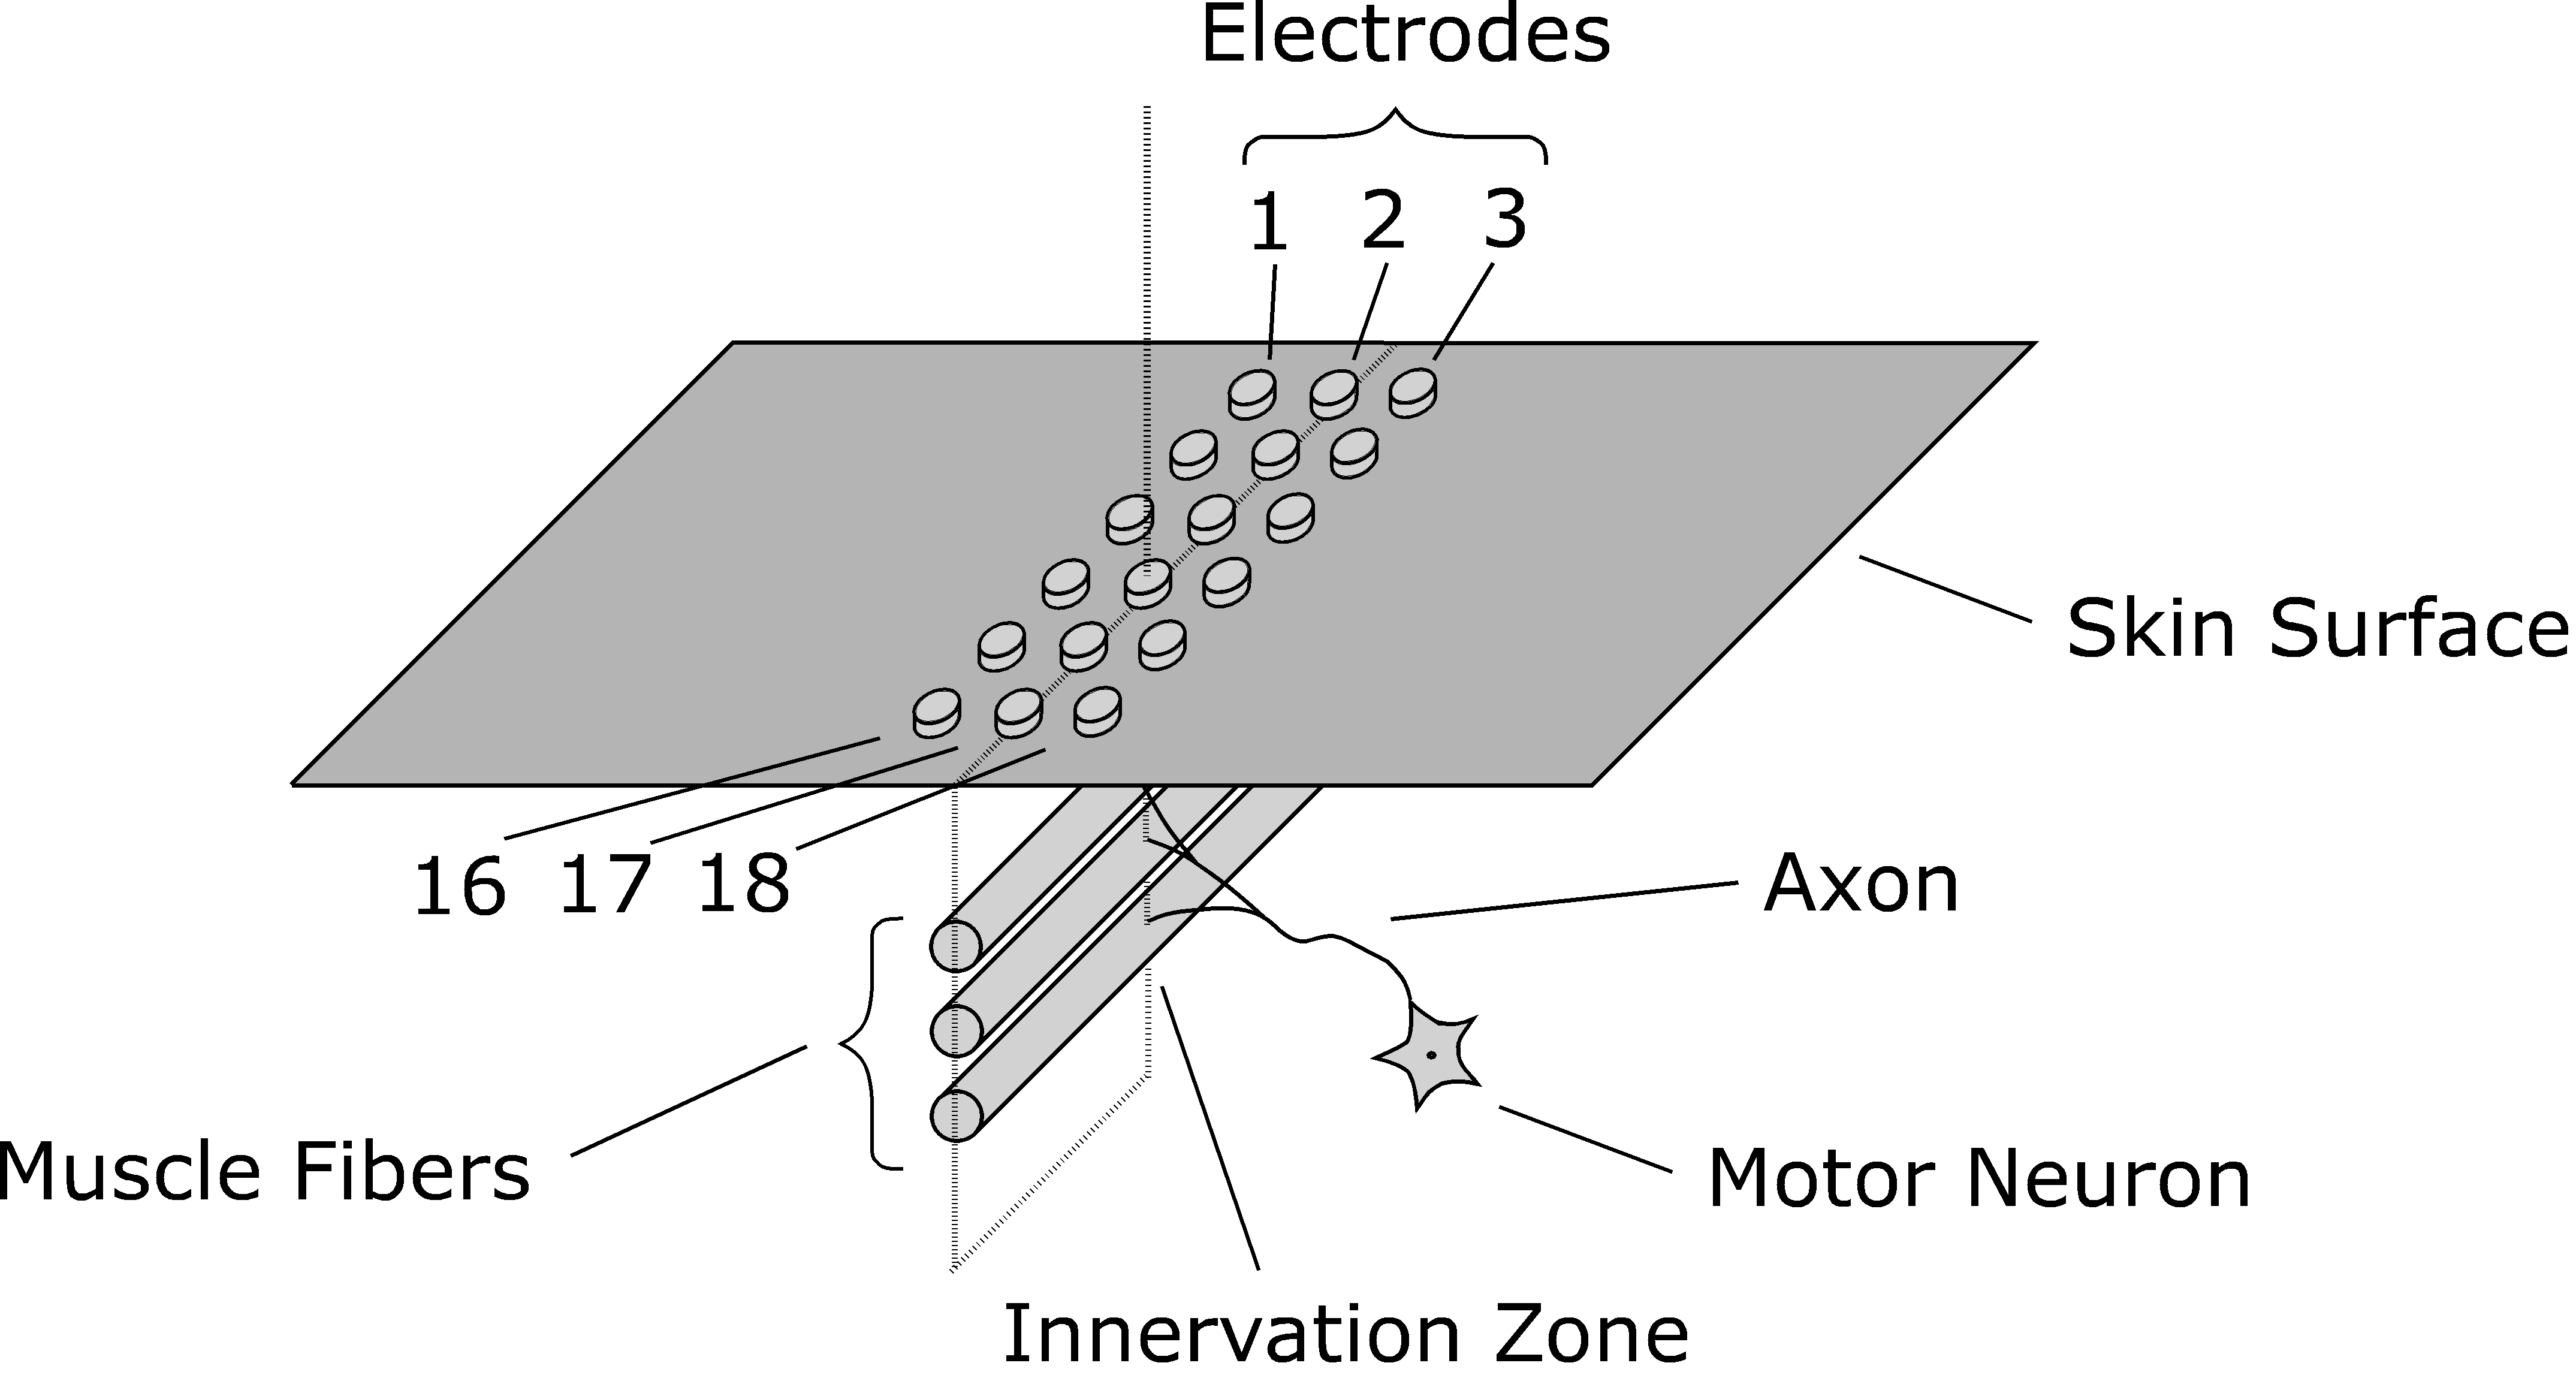
\includegraphics[width=12cm]{sfap-schematic}
  \caption[Geometry of Single Fiber Action Potential (SFAP) measurements]{Schematic of the geometry in \acrfull{sfap} measurements of human muscle fibers. Shown are three muscle fibers at different depths in the muscle tissue, and a regular grid of $18$ recording electrodes on the skin surface.}
  \label{fig:sfap-schematic}
\end{figure}

As opposed to \cref{fig:sfap-schematic}, which is included here as an external graphics file, \cref{fig:simple-schematic} shows a simple electrical schematic that is created completely in Latex, using the \swname{circuitikz} package.
\begin{figure}
  \centering
  \begin{circuitikz} \draw
    (0,0) to [V=$U_0$] (0,3)
    to [R=$R_I$, i=$I_R$] (3,3)
    to [R=$R_L$] (3,0)
    to [C=$C_P$] (0,0)
    ;
  \end{circuitikz}
  \caption{A simple electrical circuit, drawn in Latex using the \swname{circuitikz} package.}
  \label{fig:simple-schematic}
\end{figure}
This package is based on the powerful \swname{tikz} package which allows for drawing any kind of figure directly in Latex.
This bears a number of advantages:
\begin{itemize}
\item The resulting figures are vector graphics, i.e., they are small (hence not resulting in a final thesis pdf size of several MBs) and generally look good.
\item Font style and size is consistent with the rest of the document. This is a major problem when importing figures from other software, e.g., \swname{Matlab}. (Also compare \cref{fig:sfap-schematic}.)
\item Each figure created this way is completely reproducible and configurable in every aspect.
\end{itemize}
Another package that is also based on the \swname{tikz} package is the \swname{pgfplots} package which enables the user to create plots either completely in Latex, or import data from an external program (e.g., \swname{matlab}) and generate a nice-looking plot from this data using \swname{tikz} (with the advantages mentioned above).
\Cref{fig:rosenfalck} shows an example of two plots generated using the \swname{pgfplots} package.
\begin{figure}
  \centering
  \newcommand*{\scalefactor}{0.8}
  \begin{subfigure}[t]{.5\textwidth}
    \centering
    \begin{tikzpicture}
        \newcommand*{\Aros}{96}
  \newcommand*{\Bros}{-90}
  \begin{axis}[
    small,
    width = \scalefactor\textwidth,
    axis lines = left,
    x unit = mm,
    y unit = mV,
    xlabel = $z$,
    ylabel = $V$,
    xtick={0,5,10},
    ymin = -99,
    ymax = 49,
    extra y ticks = {\Bros},
    extra y tick labels = {$B$},
    ]
    % Right part of the expression
    \addplot [
    domain=-2:15, 
    samples=1000, 
    color=blue,
    ]
    {x>0 ? \Aros*x^3*e^(-x)+\Bros : \Bros};

    \draw[dashed] (-2,\Bros) -- (15,\Bros);
  \end{axis}
    \end{tikzpicture}
    \caption{$V_m(z)$}
    \label{fig:rosenfalck-1}
  \end{subfigure}%
  \begin{subfigure}[t]{.5\textwidth}
    \centering
    \begin{tikzpicture}
      \newcommand*{\Aros}{96}
\newcommand*{\Bros}{-90}
\pgfplotsset{set layers}
\begin{axis}[
  small,
  width = \scalefactor\textwidth,
  axis y line = left,
  axis x line* = bottom,
  x unit = mm,
  y unit = mV/mm,
  xlabel = $z$,
  ylabel = $\psi$,
  xmin = -15,
  xmax = 2,
  ymin = -79,
  ymax = 39,
  xtick = {-10, -5, 0},
  ]

  \addplot [
  domain=-15:2, 
  samples=1000, 
  color=blue,
  ]
  {x>=0 ? 0 : -3*\Aros*x^2*e^x-\Aros*e^x*x^3}
  node[pos = 0.03,
       pin = 70 : {$\psi$}] {};

\end{axis}

\begin{axis}[
  small,
  width = \scalefactor\textwidth,
  axis y line = right,
  axis x line = none,
  x unit = mm,
  y unit = mV/mm^2,
  xlabel = $z$,
  ylabel = $\psi'$,
  xmin = -15,
  xmax = 2,
  ymin = -59,
  ymax = 119,
  ]

  \addplot [
  domain=-15:2, 
  samples=1000, 
  color=purple,
  ]
  {x<0 ? -(6*x+6*x^2+x^3)*\Aros*e^x : 0}
  node[pos = 0.02,
       pin = 70 : {$\psi'$}] {};
\end{axis}                      

    \end{tikzpicture}
    \caption{$\psi(z)=\dd{z} V_m(-z)$ and $\psi'(z)$}
    \label{fig:rosenfalck-2}
  \end{subfigure}%
  \caption[Plots of Rosenfalck's model function for the \acrlong{iap}]{Plots of the \acrfull{iap} model function proposed by \textcite{rosenfalck69}.}
  \label{fig:rosenfalck}
\end{figure}

\section{Blind Source Separation Methods}
In this chapter in particular, you should provide a lot of references, e.g., to scientific articles~\cite{farina99}, books~\cite{plonsey07}, book chapters~\cite{rodriguez-falces12}, PhD theses~\cite{fevotte03}, or software projects~\cite{r-project} that you used during the creation of your thesis.
Sometimes, you should explicitly name authors, such as \textcite{farina99}, who wrote a seminal article on the mathematical modelling of \gls{emg} measurements.

Note how the \gls{emg} acronym is clickable and leads to the definition of this acronym in the glossary.
This is one of the many features of the \swname{glossaries} package.

\subsection{Equations}
If you are going to write more than a few equations in your thesis, it is highly recommendable to use macros to define each variable that occurs.
This way, if you decide to rename the velocity from $v$ to $v_0$ everywhere in your thesis later on during the process of writing, you will only have to change the definition of the macro used for this variable.
For example, in
\begin{equation}
  \label{eq:1}
  \vel = \frac{\diff \loc}{\diff t}
\end{equation}
and
\begin{align}
  \label{eq:2}
  \acc &= \frac{\diff \vel}{\diff t} \nonumber \\
  &= \frac{\force}{\mass}
\end{align}
each of the variables is defined using a macro.
Finally, here comes an example of how to reference equations \eqref{eq:1} to \eqref{eq:2}.

\section{Pseudo Code}
Algorithm \ref{alg:euclid} is an example of how pseudo code can be represented in Latex.
Of course there are, as with anything in Latex, many options available to achieve this goal.
Here, the \swname{algpseudocode} package is employed.
\begin{algorithm}
  % Example code due to
  % http://tex.stackexchange.com/a/230789/64293
    \caption{Euclid's algorithm}
    \label{alg:euclid}
    \begin{algorithmic}[1] % The number tells where the line numbering should start
        \Procedure{Euclid}{$a,b$} \Comment{The g.c.d. of a and b}
            \State $r\gets a \bmod b$
            \While{$r\not=0$} \Comment{We have the answer if r is 0}
                \State $a \gets b$
                \State $b \gets r$
                \State $r \gets a \bmod b$
            \EndWhile\label{euclidendwhile}
            \State \textbf{return} $b$\Comment{The gcd is b}
        \EndProcedure
    \end{algorithmic}
\end{algorithm}


%%%%% Emacs-related stuff
%%% Local Variables: 
%%% mode: latex
%%% TeX-master: "../../main"
%%% End: 

\chapter{Results}
\label{chap:results}

This chapter summarizes the results that you have obtained during experimental validation of the concept presented in the previous chapter.
Note that a clear separation between experimental results and their discussion is to be made: Here, only numerical results, performance plots, etc. are to be shown and described.
Any interpretation of these results -- What do they imply? Which conclusions do you draw? -- is to be postponed to the following chapter.
This is useful since in the future, some of your interpretations may be clearly known to be false, due to newly acquired knowledge.
In this case, however, the data you have collected during your studies may still be very valuable and hence should be easily accessible on its own.
Moreover, this provides a very important distinction between objective findings, i.e. experimental measurements that you have obtained or other data, and the inferences that you draw from these data, which may or may not be true.

%%%%% Emacs-related stuff
%%% Local Variables: 
%%% mode: latex
%%% TeX-master: "../../main"
%%% End: 

\chapter{Discussion}
\label{chap:discussion}

Finally, in this chapter, the results presented in the previous chapter are to be discussed and interpreted.
Here you may discuss the prospects of your proposed method to solve the problem at hand, and propose alternative solutions.

%%%%% Emacs-related stuff
%%% Local Variables: 
%%% mode: latex
%%% TeX-master: "../../main"
%%% End: 

\chapter{Conclusion}
\label{chap:conclusion}

In this final chapter, you provide a concise summary and conclusion of your work.

%%%%% Emacs-related stuff
%%% Local Variables: 
%%% mode: latex
%%% TeX-master: "../../main"
%%% End: 


\backmatter

% Print list of mathematical symbols
\printnoidxglossaries

\listoffigures

%\listoftables

\printbibliography

% List of fixme notes
\listoffixmes

\end{document}

%%%%% Emacs-related stuff
%%% Local Variables: 
%%% mode: latex
%%% TeX-master: t
%%% End: 
